\documentclass[12pt]{article}
\usepackage{amsmath}
\usepackage[utf8]{inputenc}
\usepackage{graphicx}
\usepackage{url}
\usepackage[font={small,it}]{caption}
%\renewcommand\familydefault{\sfdefault}
\renewcommand{\baselinestretch}{1.1}
\usepackage[letterpaper, margin=1in]{geometry}
\usepackage{listings}
\usepackage{gensymb}
\usepackage[table,x11names]{xcolor}

\lstset{basicstyle=\tiny,language=Python}

\newcommand\figref[1]{Fig.~\ref{fig:#1}}
\newcommand\secref[1]{Section~\ref{sec:#1}}
\newcommand\tabref[1]{Tab.~\ref{tab:#1}}


\title{Udacity Machine Learning Nanodegree\\ CAPSTONE: Photo OCR Prototype}
\author{Wolfgang Steiner, Dr.-Ing. \\ \small{wolfgang.steiner@gmail.com}}
\date{January 2017}

\begin{document}
\maketitle
\section{Introduction}
In this capstone project I present the prototype of a photo OCR (optical character recognition)
system based on a sliding window algorithm. The system is able to automatically detect and transcribe
digit sequences of arbitrary length in images. Systems such as this are used in a wide variety of applications
such as scanning of documents using a mobile device, automatic transcription of street signs, or
the automatic parsing of house numbers from street view photos \cite{Goodfellow2013}.

\begin{figure}
    \centering
    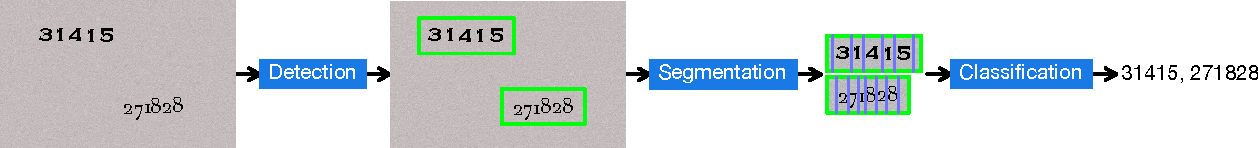
\includegraphics[scale=0.8]{fig/Pipeline}
    \caption{Photo OCR pipeline.}
    \label{fig:pipeline}
\end{figure}


The task of photo OCR can be divided into three distinct stages which are shown in \figref{pipeline}.
The first stage is \emph{text detection} which aims to determine bounding boxes for each
distinct set of characters in the image. The second stage is \emph{character segmentation}, in which
each bounding box is scanned for character boundaries with the aim of finding distinct characters
that can finally be classified in the third stage by the \emph{character classification}.
The implementation of the three classifiers is based on convolutional neural network (CNN)
architectures that have been trained exclusively on synthetic text images (similar to \cite{Jaderberg2016}).
In order to reduce the complexity and training time of the project, the pipeline is confined to
only process and transcribe digits, but every stage could in principle be extended and retrained
to also handle all the characters of the alphabet.


As part of this project, a real-time demo has been implemented that successfully detects
and transcribes digit sequences in the video stream provided by a webcam. While requiring
a GPU for operation, this prototype demonstrates that it is possible to train an OCR system
with synthetic data only, which greatly simplifies the development process.


\section{Metrics and Benchmark}
\label{sec:metrics}
In order to assess the performance of the complete OCR pipeline, a set of test images $x_i$ containing
a randomly generated string of digits of varying length is processed and the extracted string $a(x_i)$ is
compared to the real label $y(x_i)$ using the following metric:
\begin{equation}
  \operatorname{accuracy}(\begin{bmatrix}x_{1}\\x_{2}\\\vdots\\x_{n}\end{bmatrix},\begin{bmatrix}y(x_{1})\\y(x_{2})\\\vdots\\y(x_{n})\end{bmatrix}) = 1 - \frac{\sum\limits_{i=0}^n{\operatorname{min}\left(\operatorname{lev}(y(x_i), a(x_i)), |y(x_i)|\right)}}{\sum\limits_{i=0}^n{|y(x_i)|}}
\end{equation}
Here, $a(x_i)$ is the label (string of digits) predicted by the system and $|y(x_i)|$ is the length of
the i-th true label. $\operatorname{lev}(y(x_i), a(x_i))$ denotes the Levenshtein distance \cite{Levensht20:online} between
the true label and the predicted label, which counts the number of edit operations
that are required to make two strings exactly equal by either deleting, inserting or
changing single characters. When calculating the accuracy, the Levenshtein distance is limited to
the length of the true label (by use of the $\operatorname{min}$ function). This prevents the accuracy
of a single example to become negative.

Human level performance on the task of text transcription is often estimated to be greater
than 98\% \cite{Goodfellow2013}. So an obvious benchmark for a OCR system would be to
attain comparable or even better performance than a human is capable of. When extracting words,
the performance of the system can be augmented by use of a dictionary to correct badly classified
characters. When dealing with number strings only, this augmentation is not possible and
the accuracy of the OCR system is a direct measurement of performance.

A second performance benchmark is speed. One application for an OCR system would be text extraction
of documents scanned by use of the camera of a smartphone. The images would then be send to
a server for processing or, even better, would be precessed directly on the mobile device.
In both cases scanning a photo for text should not take more than a few seconds. For use in
an augmented reality app, the speed needs to be even faster in order to allow for an acceptable
frame rate. In this case, processing on the mobile device should be faster than about
250ms.

\newpage
\section{Training Data}
In this project I exclusively used synthetic images to train the three CNN classifiers
of the OCR pipeline. In order to have a large variety of fonts,
I used the google fonts repository as a source \cite{googlefo53:online}. After excluding some
symbol and non-latin fonts, a collection of 1747 fonts was available for synthesizing images.
The procedure for synthesizing training images is as follows:

\begin{figure}[b!]
  \centering
  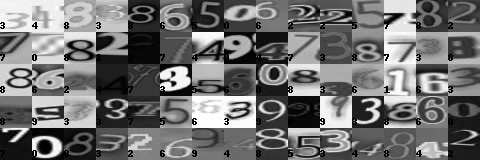
\includegraphics[width=1.0\linewidth]{fig/training_example_images/classifier}
  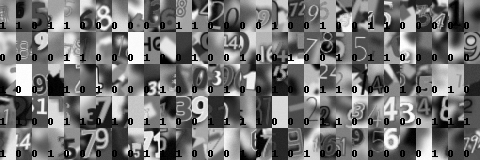
\includegraphics[width=1.0\linewidth]{fig/training_example_images/segmentation}
  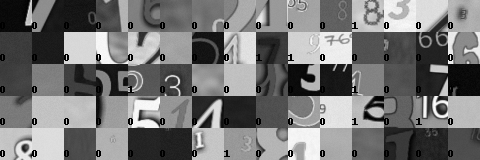
\includegraphics[width=1.0\linewidth]{fig/training_example_images/detection}
  \caption
  {
    Examples of synthesized images used to train the character classifier (top),
    character segmentation classifier (center) and character detection classifier (bottom).
  }
  \label{fig:training_images}
\end{figure}

\begin{itemize}
  \itemsep0em
  \item A text and a background color is chosen randomly.
  \item A background image is synthesized by upscaling noise by a random factor and applying gaussian blurring.
  \item One of the 1747 fonts is chosen randomly.
  \item One of the characters is chosen randomly.
  \item Adjacent characters are added in some images to the left or right.
  \item An outline is randomly added to the characters.
  \item A shadow of random width and direction is added to the characters.
  \item The image is rotated by a random amount.
  \item Gaussian blur is applied with random radius.
  \item White noise of random amount is added to the image.
\end{itemize}



Some examples of images used to train the three required CNN classifiers are shown in \figref{training_images}.
In all cases, training and prediction is done with grayscale images with a fixed height of 32~pixels.
Training images are not pre-generated before training but are synthesized online during training,
which allows for a virtually unlimited number of unique images.
For this I implemented python generators for the three types of training images that synthesize
batches of images in separate worker threads.

Training images for the character classifier (\figref{training_images}, top) have characters centered in the images (32x32~pixels) as will be encountered
by the classifier after segmentation.
%
Characters are also resized to the width of the image as the windows between character boundaries are rescaled to the
input width of 32~pixels.
%
The labels are simply the corresponding character and are one-hot encoded for training and prediction.


Training images for the segmentation classifier (\figref{training_images}, center) are only 16~pixels wide in order to improve the spatial resolution of the segmentation procedure (see below).
%
Here, label "1" is assigned if a character starts to the right of the center (for the beginning of a character sequence),
a character starts to the left of the center (for the end of a character sequence), or if the spacing
between characters is in the center of the image (for segmenting between characters of a sequence).
%
Label "0" is assigned, if no character is present in the image or if a character is in the center of the image.


Finally, the training images for the character detection classifier (\figref{training_images}, bottom) are
designed to find bounding boxes for character sequences that fit as tightly as possible in order to improve
the accuracy of character segmentation and classification.
%
Because of this, only images that contain complete or nearly complete characters are labeled
as "1". Images that contain very small characters or only parts of very large ones, as well
as images that do not contain characters are labeled "0" by the algorithm.

\section{Algorithms and Techniques}
\subsection{Text Detection}
\label{sec:detection_algorithm}
The first step in the OCR pipeline is text detection.
%
Here, a two dimensional sliding window algorithm with a window size of 32x32~pixels is used to detect characters in the image and to fit bounding boxes
around each character sequence encountered. The position of the sliding window is updated by the
following rule, where $w$ is the width of the window and $\delta_w$ is a hyper-parameter of the
algorithm, that determines the overlap between succeeding window evaluations and thus the
spatial resolution:

\begin{equation}
  x_{i+1} = x_i + \frac{w}{\delta_w}
\end{equation}

In order to detect text of different sizes, the process of sliding windows is repeated at different
image scales. The scaling factor $\alpha_i$ for iteration i is determined by:

\begin{equation}
  \alpha_i = \alpha_{max} * (\delta_\alpha)^i  \ge \alpha_{min}
\end{equation}

The factor $\delta_\alpha$ is a second hyper-parameter of the algorithm and determines the
resolution of the algorithm with respect to different text sizes.
The choice of $\alpha_{max}$ and $\alpha_{min}$ directly determines the
smallest/biggest size of text that can be recognized and processed by the following stages of the
pipeline.
When scaling the image for one iteration of the sliding window procedure, it is also rescaled
so that its width and height are multiples of 32~pixels, which is the input size of the character detection
classifier.

The image data of each window is then concatenated into an input tensor for the character detection
classifier which has a sigmoid activation function at its output.
If the predicted value for a window exceeds a certain threshold $\theta_r$
it is added to a rectangle list for further processing. After iterating over all of the
scaling steps, the unions of mutually overlapping rectangles are computed.
At the end of the procedure, each union of positively classified rectangles is likely to be a bounding
box containing a character sequence which is subsequently segmented into single characters for classification.

In order to improve performance, a very simple CNN classifier has been trained for text detection (\figref{detection_cnn}).
It consists of two convolutional layers with rectified linear units (ReLU) as activations. After
each convolutional layer, a max pooling layer reduces the size of the tensor by a factor of two in
both image dimensions.
The flattened output of the last pooling layer is then fed into two fully connected hidden layers
with 128 output neurons each. Again, ReLU is used as activation. The output layer has just one
output neuron and has a sigmoid activation layer following it. The output value of the network
will approach zero if the respective input window does not contain text and one if it does.

\begin{figure}[ht]
  \centering
  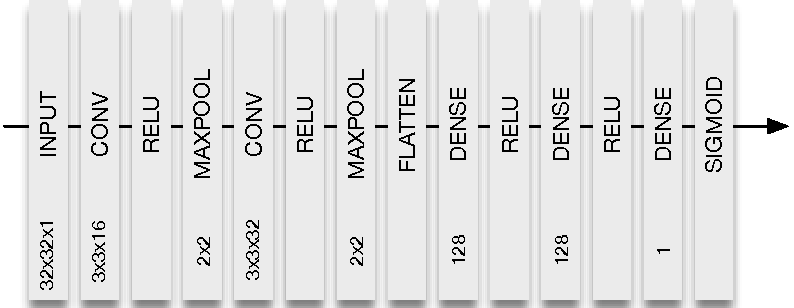
\includegraphics[scale=0.75]{fig/Detection_CNN}
  \caption
  {
    Convolutional neural network architecture of the character detection classifier.
  }
  \label{fig:detection_cnn}
\end{figure}

\subsection{Character Segmentation}
\label{sec:segmentation_algorithm}
Character segmentation is based on a one-dimensional sliding window algorithm. In order to
increase the spatial accuracy of the algorithm and to reduce the number of false positives
for very narrow characters, the width to the sliding window is halved to 16~pixels in comparison
to the text detection window, while the height remains equal at 32~pixels.

In a first step, the text bounding box to be processed is proportionally rescaled to a height of 32~pixels.
Then, in order to reliably detect the first and final character borders, even if the first/last
characters are close to the left/right borders of the bounding box, the image is extended by
half of the segmentation window's width (8~pixel) on the left and right side by repeating the first/last
pixel column.

The segmentation window is then moved with a one pixel increment from the left towards the right
edge of the rescaled bounding box. At every iteration, the pixel data of the window is concatenated
into an input tensor for the character segmentation CNN classifier. After evaluating the
tensor, a vector is obtained which has the score of range $[0,1]$ of the classifier's sigmoid output activation
for each pixel of the sliding window iteration.

In order to reduce the number of false positives, the segmentation score is then filtered by
a simple first order IIR filter \cite{Infinite55:online} with a filter constant of $0.5$. On this
filtered score, a simple peak detection algorithm finally locates the character boundaries at
the center of the pixel intervals whose activation exceeds a certain threshold
(activation threshold $\theta_s$). Examples of the results of this technique are shown
in \figref{segmentation}.

\begin{figure}[ht]
    \centering
    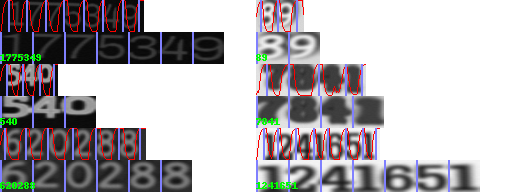
\includegraphics[width=1.1\linewidth]{fig/segmentation}
    \caption{
      Example results of the character segmentation algorithm. The top row of each example shows the input
      image. The filtered activation of the segmentation classifier is visualized in red,
      while the inferred character boundaries are marked in light blue.
      The bottom row shows the character images that have been extracted and rescaled based on the
      segmentation. These 32x32~pixel sized images are then fed into the character classifier. }
    \label{fig:segmentation}
\end{figure}

The architecture of the CNN classifier used for segmentation is shown in \figref{segmentation_cnn}.
In comparison to the text detection classifier, the network had to be extended in order
to achieve an acceptable segmentation accuracy. It consists of six convolutional layers
with ReLU activation with max pooling layers after each second layer. The two fully connected
hidden layers also where doubled in size. The output layer, again, has one output neuron
with sigmoid activation. The increased complexity of this classifier does not have as
great an impact on performance because it is only evaluated on the final rescaled text bounding boxes
and not on the whole input image.

\begin{figure}[ht]
  \centering
  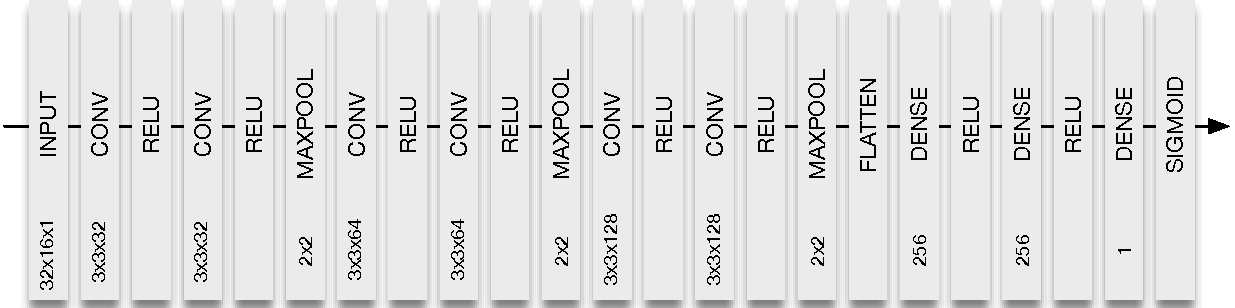
\includegraphics[scale=0.75]{fig/Segmentation_CNN}
  \caption
  {
    Convolutional neural network architecture of the character segmentation classifier.
  }
  \label{fig:segmentation_cnn}
\end{figure}



\subsection{Character Classification}
In comparison, the final stage of the OCR pipeline is rather straight-forward. At this point
in time, a list of character boundaries is available for each text bounding box. From this list,
the pixel data for each character candidate is rescaled to an image of size 32x32~pixels and
normalized to values of range $[0,1]$.

The architecture of the character classifier is shown in \figref{classifier_cnn} and is
quite similar to the segmentation classifier. The structure of the convolutional layers is
identical (apart from the different shape of the input tensor), while the size of hidden
fully connected layers has been increased substantially in order to allow for the
classification of the ten distinct digits. Accordingly, the output layer has an output size
of ten and has a softmax activation function. The output of this network is a vector
with ten entries which can be interpreted as the probabilities for the ten different classes.

\begin{figure}[ht]
  \centering
  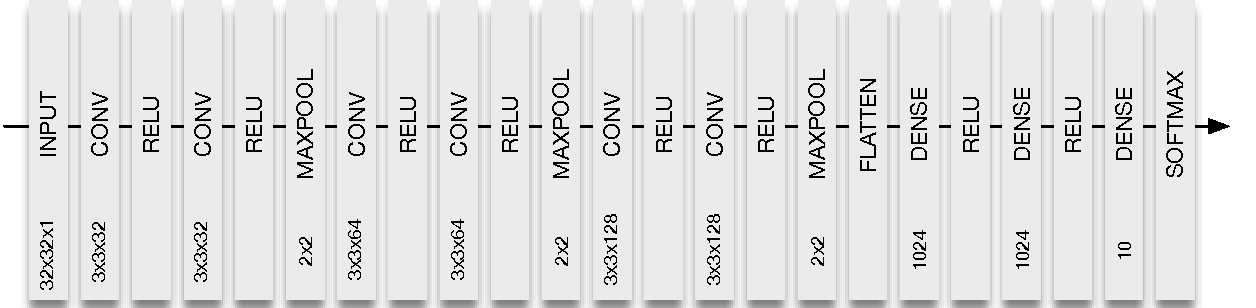
\includegraphics[scale=0.75]{fig/Classifier_CNN}
  \caption
  {
    Convolutional neural network architecture of the character classifier.
  }
  \label{fig:classifier_cnn}
\end{figure}


\section{Methodology}
In order to implement the OCR system, I followed a bottom-up approach. First, I implemented
the character generator capable of synthesizing training images (\figref{training_images}, top)
for the character classifier (\figref{classifier_cnn}). In order to facilitate easy and rapid
experimentation, I also implemented a simple front-end DSL based on keras \cite{KerasDoc40:online} that allows
for concise and expressive definitions of CNN architectures. This greatly simplified the
process of finding a suitable CNN architecture which started with a simple model with only
two convolutional layers that was successively extended by adding more convolutional layers
and increasing their filter depth until reaching the final architecture in \figref{classifier_cnn}.

Training data is synthesized online during training on multiple CPU threads, using a keras generator. The classifier was trained
on a GPU (GTX~1080) using the Adam optimizer \cite{Kingma2014} and a batch size of 128.
Preprocessing simply involved normalizing the pixel values to a range of $[0, 1]$ and one-hot encoding
the labels. The epoch size is set to a rather high value of $2^{17}$,
which results in a training time of about one minute per epoch on the GPU.
After each epoch, the accuracy and categorical cross-entropy loss on a validation set of
2048 pre-generated images is calculated.
The learning rate is empirically set to the highest value that still results in fast initial training progress and is then
successively reduced whenever the validation loss does not improve for more than four epochs.

One big advantage of training the classifier from randomly generated data is that overfitting
is effectively avoided as each training example is uniquely synthesized. Because of this,
regularization measures such as dropout \cite{Srivastava2014} or weight regularization proved not to be essential
in order to train a model that generalizes well. Another advantage is that it easily becomes
possible to overtrain the classifier with data that is more demanding than the one it will
encounter during deployment. Here, training examples are generated that have a higher degree
of blurring (max radius of 2.5 vs.\ 1.5) and that are rotated further from the upright position
($\sigma=15\degree$ vs.\ $\sigma=7.5\degree$)
than will probably be encountered as part of the OCR system.

%\lstinputlisting[float,caption={Implementation of the character classifier CNN.},label={listing:classifier_cnn}]{../train-classifier.py}

\begin{figure}[t!]
  \centering
  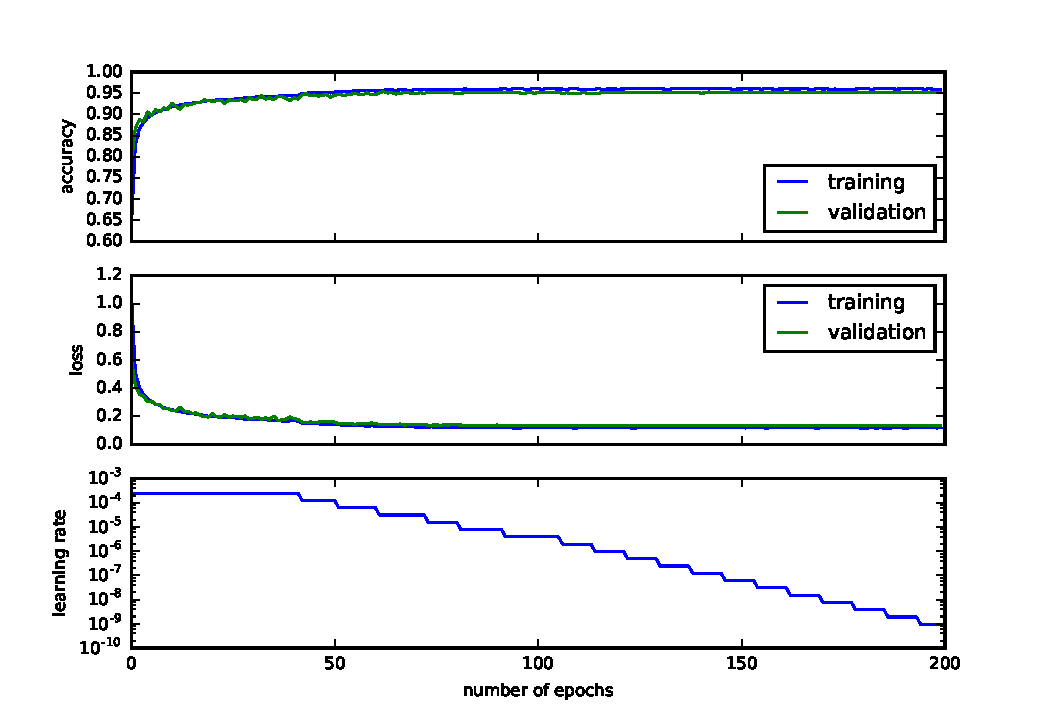
\includegraphics{fig/learning_curve}
  \caption{
    Learning curves for training of the character classifier:
    accuracy (top), loss (center) and learning rate (bottom) plotted as functions of
    the number of epochs.
    \label{fig:learning_curve}
  }
\end{figure}

In order to monitor training progress and also to compare training of different CNN architectures,
I made extensive use of learning curves like the one shown in \figref{learning_curve}.
Here, accuracy and loss are compared both for the training and the validation set as functions
of the number of epochs. Note that in this case, both the test and the validation accuracy
have very similar values throughout the training process,
which shows that overfitting is effectively avoided through
the use of randomly synthesized training data. Also plotted in \figref{learning_curve} (bottom)
is the learning rate. It can be clearly seen how the learning rate is reduced successively
whenever the validation accuracy fails to improve further.

After training for 200 epochs and about six hours, the learning rate has been reduced to $\approx 10^{-9}$ and training progress
has effectively ceased. Evaluating a randomly generated test set of 8192 characters yields
an accuracy of 98.16\%. In order to further justify the above described training methodology,
the character classifier was used to evaluate the test set of the google street view house numbers dataset
\cite{Netzer2011,TheStree9:online}. Some examples from this dataset are show in \figref{svhn_data}.
The dataset consists of 26032 images that were cropped from photos taken by the
google street view project and are evidently of a very challenging quality, with many examples that are heavily blurred to a
degree that would not be encountered by an OCR system. Despite this, the character classifier
achieves an accuracy of 83.83\% after training only on synthetic data.

\begin{figure}
  \centering
  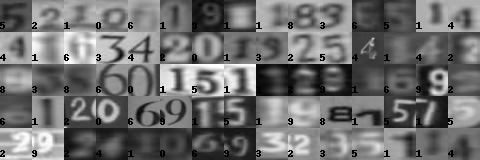
\includegraphics[width=1.0\linewidth]{fig/svhn_test}
  \caption
  {
    Example images from the google street view house numbers test dataset \cite{Netzer2011,TheStree9:online}.
  }
  \label{fig:svhn_data}
\end{figure}

In a second step, I started to work on character segmentation. For this, new training
data was needed: the character segmentation classifier's output should have a high
activation when the gap between two characters is present in the center of its
16x32~pixel input window and, conversely a low activation when a character is in the
center of the window or if no character is present at all.
Accordingly I implemented a variation of the character generator that will generate
randomly synthesized images with these specifications (cf.~\figref{training_images}, center).

The CNN segmentation classifier (cf.~\figref{segmentation_cnn}) was trained in a very similar way as described above for the
character classifier. Testing the fully trained segmentation classifier on a test dataset consisting
of 8192 randomly generated segmentation examples results in an accuracy of 95.04\%.
As for the character classifier, the segmentation classifier was also trained on examples
that were blurred to a higher degree (blur radius of 2.5 vs.\ 1.5) and were rotated at a higher
maximal angle ($\sigma=15\degree$ vs.\ $\sigma=7.5\degree$) than would be expected in deployment, thus
yielding a higher test accuracy than for the validation set (90.28\%).

After implementing the sliding window algorithm for character segmentation discussed in
\secref{segmentation_algorithm}, the performance of character segmentation and classification
working together could be tested for the first time. For this, I implemented a generator
for creating images of random digit strings with a height of 32~pixels.
Some examples of these test images, together with the filtered activation of the
segmentation classifier and the resulting
character boundaries and input images for classification were already shown in
\figref{segmentation}. After optimizing the hyper parameters of the segmentation algorithm
(activation threshold $\theta_s$ and activation filter constant), the segmentation/classification
achieved an accuracy of 97.04\% on a test set of 8192 randomly generated text images.
The accuracy was calculated using the Levenshtein distance between each predicted digit
string and ground truth, as discussed in \secref{metrics}.

The final step of implementing the OCR pipeline was now to tackle text detection.
Again, a generator for training images was needed to train the CNN detection classifier.
In order to calculate text bounding boxes that fit the enclosed text as closely as possible
in the vertical direction, training images are labeled "1" if a digit is fully or at least
nearly fully visible. If the digits are very small, however, the respective image is labeled
"0". All images that do not contain any digits or that only contain parts of very big digits
are labeled "0" as well. The last property is important in order to make text detection
more resilient against edges in the source image that do not belong to any digits.
For examples of training images, see \figref{training_images}, bottom.

After training the text detection classifier (cf.~\figref{detection_cnn}) for 200 epochs,
it achieves an accuracy of 94.47\% on a test set of 8192 randomly generated detection examples.
With the fully trained text detection classifier I then proceeded to implement the
text detection algorithm described in section \secref{detection_algorithm}. For the system
to perform at its peak performance, the hyper parameters $\delta_\alpha$, $\delta_w$ and $\theta_r$
had to be determined by performing a grid search. For this, a test set of 100 images of size 640x480~pixels
where randomly generated. The results of the grid search are summarized in Tab.~\ref{tab:gridsearch}.


\begin{table}[b!]
\centering
\caption{Results of a grid search on the hyper-parameters $\delta_\alpha$, $\delta_w$ and $\theta_r$
of the text detection algorithm described in \secref{detection_algorithm}.
Evaluation was performed on a test set consisting of 100 randomly generated images of digit strings.}
\label{tab:gridsearch}
\footnotesize
\begin{tabular}{|c|c|c|c|r|}
\hline
\rowcolor{lightgray}$\delta_\alpha$ & $\delta_w$ & $\theta_r$ & accuracy & time \\
\hline
0.5000  &  4.0  &  0.750  &  61.99\%  &  60s \\
0.6250  &  4.0  &  0.750  &  89.59\%  &  66s \\
\rowcolor{Honeydew2} {\bf 0.7500}  &  4.0  &  0.750  &  93.21\%  &  81s \\
0.8750  &  4.0  &  0.750  &  92.76\%  & 124s \\
0.9375  &  4.0  &  0.750  &  92.53\%  & 211s \\
\hline
0.7500  &  2.0  &  0.750  &  74.89\%  &  42s \\
0.7500  &  2.5  &  0.750  &  86.65\%  &  48s \\
0.7500  &  3.0  &  0.750  &  89.14\%  &  61s \\
\rowcolor{Honeydew2} 0.7500  &  {\bf 4.0}  &  0.750  &  93.21\%  &  81s \\
0.7500  &  6.0  &  0.750  &  92.08\%  & 156s \\
0.7500  &  8.0  &  0.750  &  92.53\%  & 231s \\
\hline
0.7500  &  4.0  &  0.500  &  93.21\%  &  82s \\
\rowcolor{Honeydew2} 0.7500  &  4.0  &  {\bf 0.625}  &  94.34\%  &  81s \\
0.7500  &  4.0  &  0.750  &  93.21\%  &  81s \\
0.7500  &  4.0  &  0.875  &  89.14\%  &  80s \\
0.7500  &  4.0  &  0.950  &  78.28\%  &  80s \\
0.7500  &  4.0  &  0.980  &  60.86\%  &  80s \\
\hline
\end{tabular}
\end{table}

Finally, I implemented a small demo app that uses the OCR system to detect and transcribe
digit strings in the video stream provided by a webcam. Video frames captured using
the OpenCV \cite{OpenCVOp84:online} module are preprocessed by converting to grayscale and
normalizing the pixel values to the range $[0,1]$. The maximum and minimum scale
factors for the text detection algorithm are determined based on the resolution of the
input image and the image is then processed by the OCR pipeline. Detected and transcribed
digit strings are then annotated in the original image. To reach a more or less acceptable
performance I had to make some compromises like skipping a number of frames and reducing
the pipeline's accuracy by decreasing the window overlap during text detection ($\delta_w$).
With these measures I was able to get acceptable frame rates when running on a GPU.


\section{Results}
In order to assess the performance of the completed photo OCR system, images of random digit sequences
of size 640x480~pixels where generated with random backgrounds, random fonts, random outlines,
random shadows, random rotation and random blurring. Some examples of correctly detected and
transcribed digit sequences are shown in \figref{good_examples_pipeline}. Here, positively
classified windows of the text detection algorithm are drawn in red with the resulting
text bounding box drawn in green. The digit boundaries found by the character segmentation
algorithms are drawn in light blue. Examples of incorrectly transcribed sequences are
shown in \figref{bad_examples_pipeline}. In some cases, the bounding box is not correctly
inferred (top, left), in other cases not all character boundaries are detected correctly.
The algorithm struggles most when the text is rotated by a large angle when the segmentation
algorithm starts to fail.

\begin{figure}[b!]
    \centering
    \makebox[\textwidth][c]
    {
        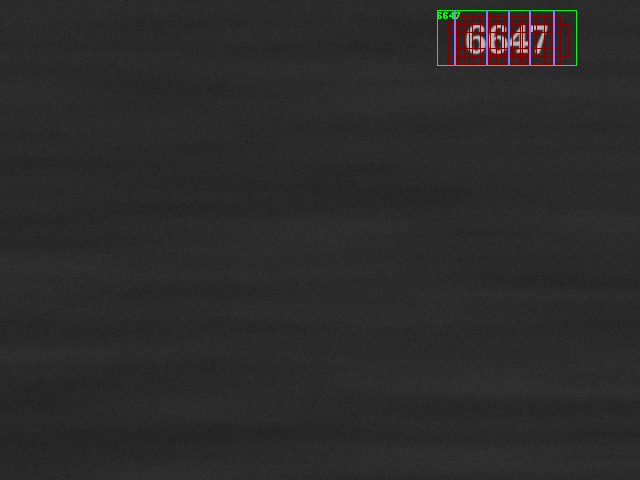
\includegraphics[width=0.35\linewidth]{fig/good_examples_pipeline/18efed02-10b7-47ce-af1e-e74a96365ea2}
        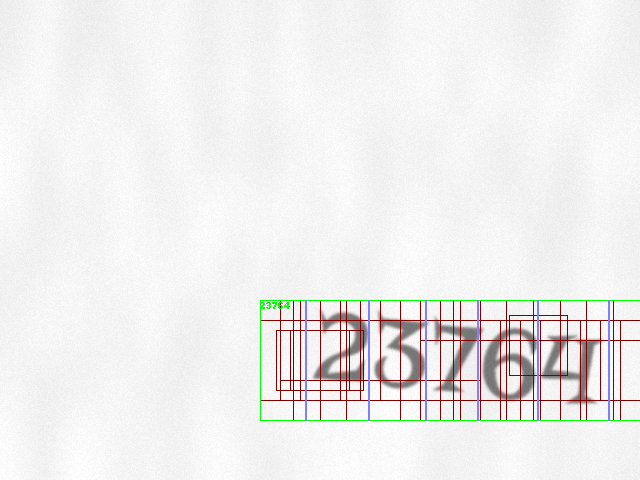
\includegraphics[width=0.35\linewidth]{fig/good_examples_pipeline/5c90c282-78f7-4432-acb0-38f245162ea9}
        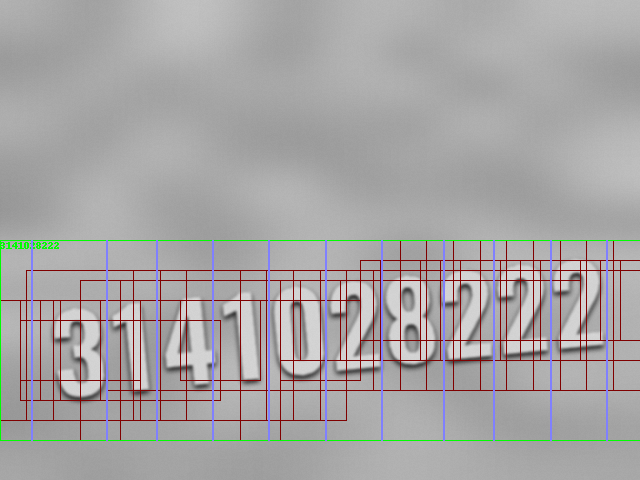
\includegraphics[width=0.35\linewidth]{fig/good_examples_pipeline/748022aa-dc7c-42d6-951b-a57db43b46b0}
    }
    \makebox[\textwidth][c]
    {
        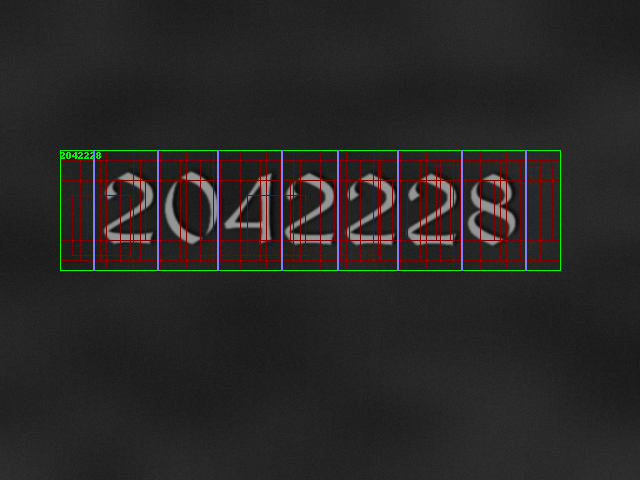
\includegraphics[width=0.35\linewidth]{fig/good_examples_pipeline/7c3ca18f-4366-40b6-8fc3-40ca42834fb9}
        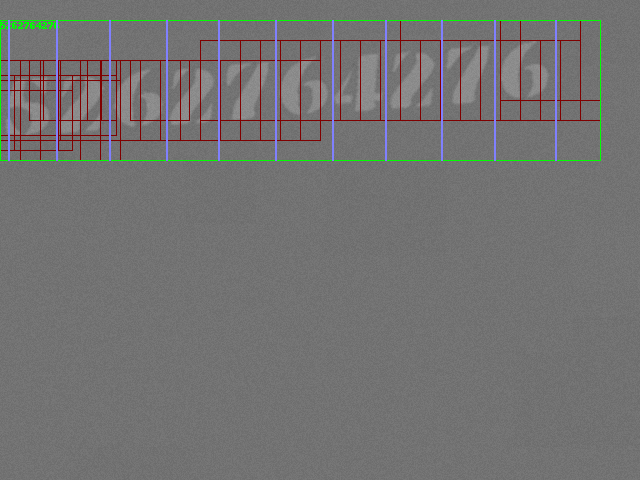
\includegraphics[width=0.35\linewidth]{fig/good_examples_pipeline/91596cec-4621-4e28-bc14-04e4815b52f9}
        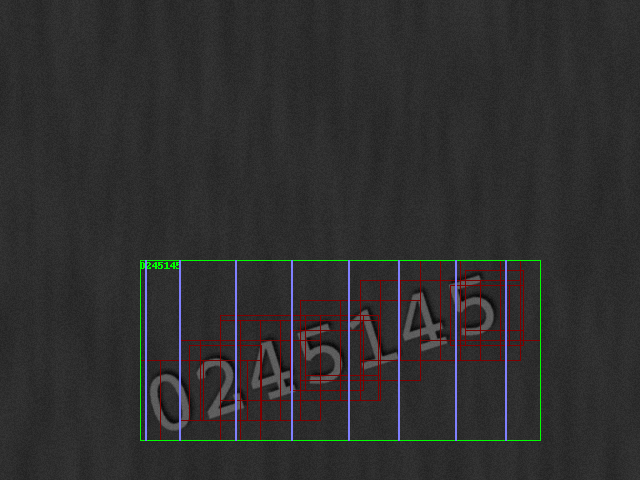
\includegraphics[width=0.35\linewidth]{fig/good_examples_pipeline/c572f505-791b-45be-bf60-9761fd9eb1b6}
    }
    \caption{Examples of correctly transcribed digit strings. Red rectangles are positive classifications of the
    character detection classifier. The green rectangles corresponds to the bounding boxes calculated as the union
    of the red rectangles. Boundaries between characters, inferred by the segmentation algorithm, are drawn in light blue.}
    \label{fig:good_examples_pipeline}
\end{figure}

\begin{figure}[t]
    \centering
    \makebox[\textwidth][c]
    {
        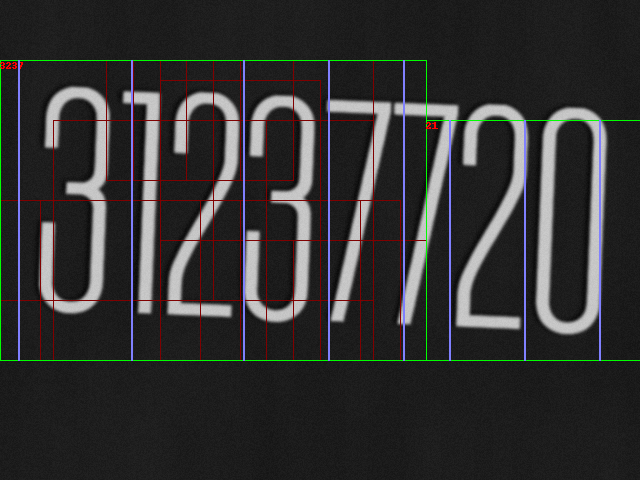
\includegraphics[width=0.35\linewidth]{fig/bad_examples_pipeline/81bde1bf-e51e-4a21-8dff-2928d5d48130}
        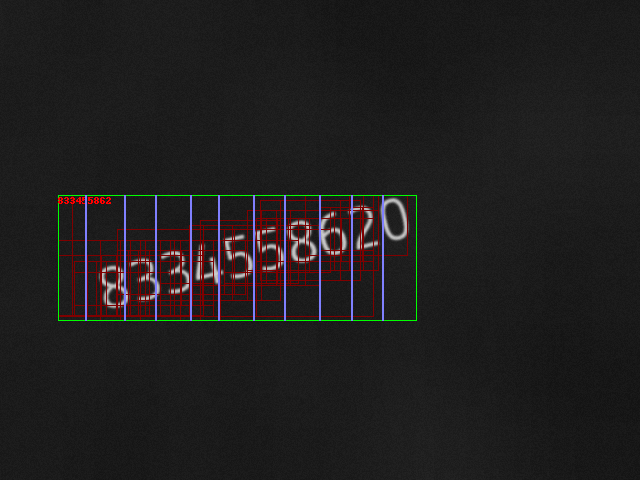
\includegraphics[width=0.35\linewidth]{fig/bad_examples_pipeline/9a566395-02bf-4676-8134-83296ded2838}
        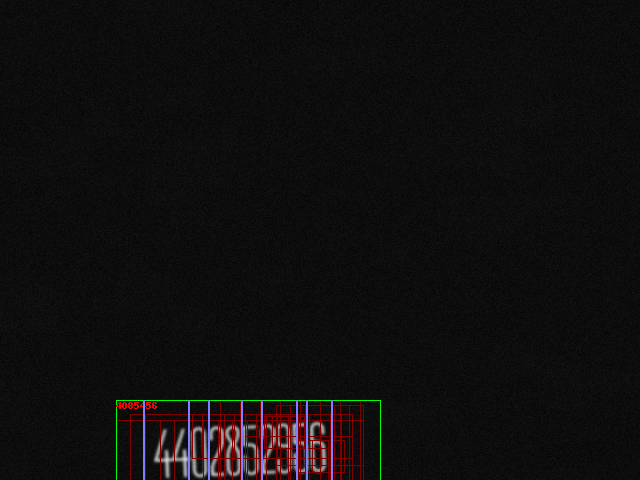
\includegraphics[width=0.35\linewidth]{fig/bad_examples_pipeline/ab748dac-6dea-41e4-9780-db48e996fd6b}
    }
    \makebox[\textwidth][c]
    {
        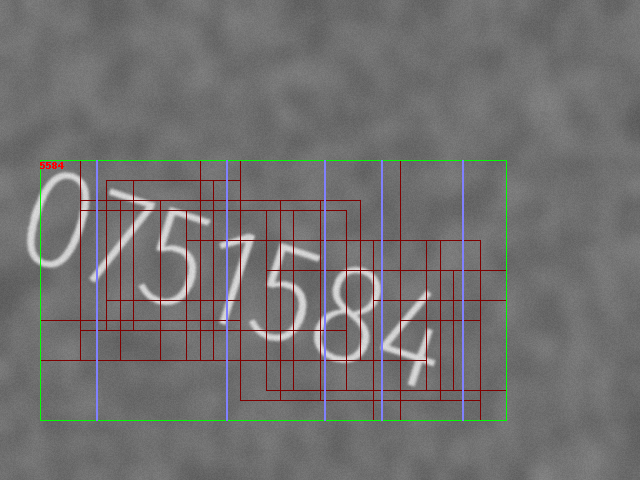
\includegraphics[width=0.35\linewidth]{fig/bad_examples_pipeline/a29de7ae-0adc-4527-b349-a317c29a6d16}
        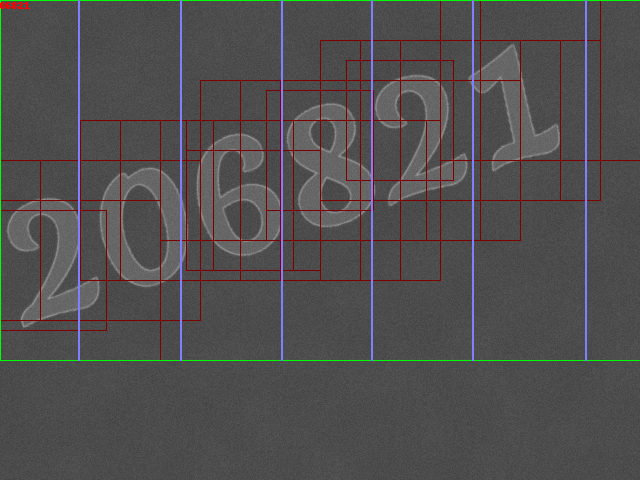
\includegraphics[width=0.35\linewidth]{fig/bad_examples_pipeline/f063436b-3b07-4987-969b-2ce211ad4449}
        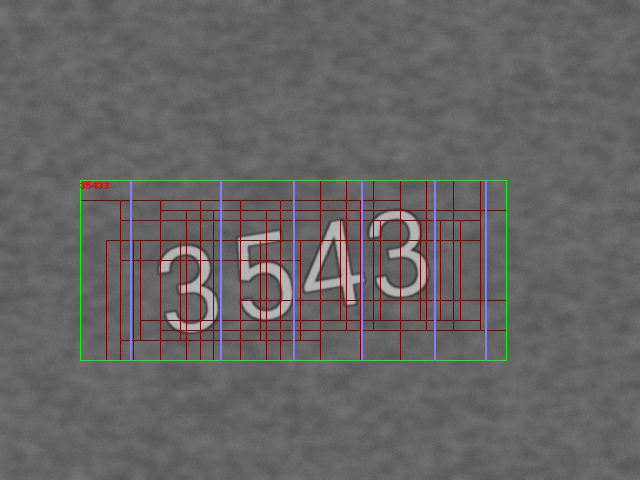
\includegraphics[width=0.35\linewidth]{fig/bad_examples_pipeline/cc904d6d-5202-422b-9a31-e8e49ddad840}
    }
    \caption{
      Examples of incorrectly transcribed digit strings. Repetition of digits (left).
      Missing digits (center). Low contrast images and small test size may result in character failing detection,
      resulting in a bounding box that is too small for segmentation and classification (right).
    }
    \label{fig:bad_examples_pipeline}
\end{figure}


\begin{table}[h!]
\centering
\caption{Accuracy of the OCR system on four different test sets of 512 randomly generated
digit sequence images (size 640x480~pixels). The experiments were conducted on a GTX~1080 GPU.
Starting from a baseline set, one set with more blurring, one with greater rotation and
one blurred and rotated test set were evaluated.}
\label{tab:results_ocr}
\footnotesize
\begin{tabular}{|l|c|c|c|c|c|}
\hline
\rowcolor{lightgray} Test Set & max. blur radius & $\sigma$ rotation & accuracy     & time \\
\hline
baseline       &   1.5            & 2.5               & 94.09\%    &  419s \\
blur           &   4.0            & 2.5               & 93.48\%    &  420s \\
rotate         &   1.5            & 7.5               & 87.46\%    &  409s \\
blur + rotate  &   4.0            & 7.5               & 85.47\%    &  409s \\
\hline
\end{tabular}
\end{table}


The results of testing the OCR system on four different sets of images are summarized in
\tabref{results_ocr}. For images containing mostly horizontal text with a random rotation
following a gaussian distribution with $\sigma = 2.5\degree$ and only light blurring
('baseline') the system achieves an accuracy of 94.09\% (using the Levenshtein distance as
defined in \secref{metrics}). While not quite reaching human performance, this is still
quite encouraging! Regrettably, the algorithm takes $\approx 820~ms$ per image on a
GTX~1080, which is a high-end GPU.

As can be expected, accuracy degrades when the source images are blurred (93.48\%) and
especially when the text is not aligned horizontally (87.47\%). When combining both
blurring and rotation, the system still detects and classifies 85.47\% of all digits
correctly.

As part of this project a proof-of-concept demo was implemented that detects and transcribes
strings of digits using a webcam. Example screenshots of this demo in action are shown in \figref{webcam}.
As can be seen, the system works in principle and successfully detects and transcribes
horizontally aligned digit sequences (top left) but decreases in accuracy for rotated
text (top right). It shows some resiliency against clutter in the image (bottom left) and even manages
to successfully transcribe a handwritten digit sequence (bottom right) in some cases.
Regrettably, performance is lacking: even when running the OCR pipeline on a mid-range GPU (GTX 1060),
the system struggles to deliver an acceptable frame rate.

\begin{figure}[ht]
    \centering
    \makebox[\textwidth][c]
    {
      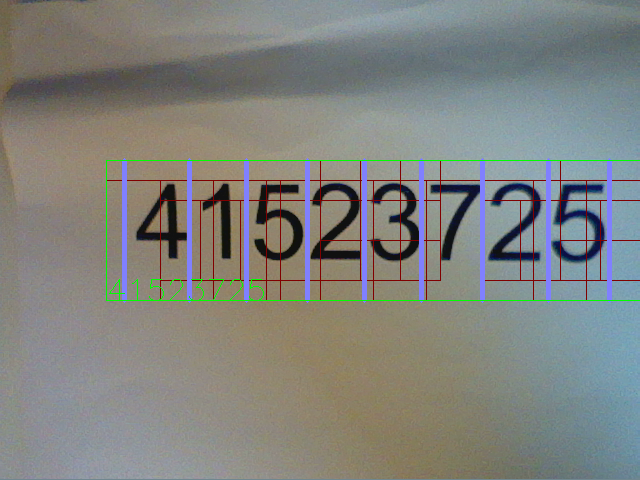
\includegraphics[width=0.5\linewidth]{fig/screenshots/eee8d50a-684a-4f54-8e89-3c4e729530c1}
      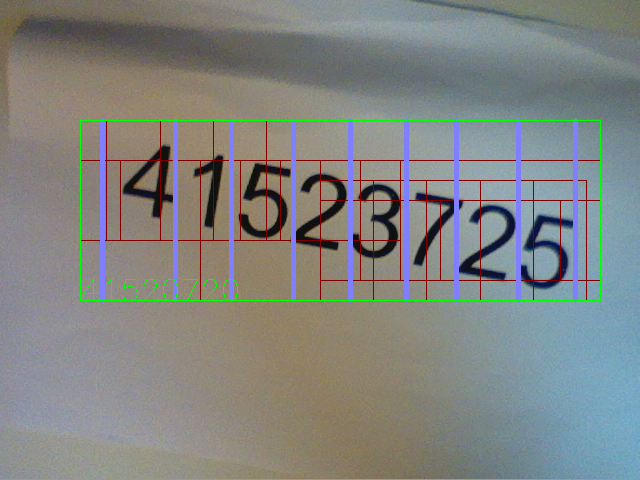
\includegraphics[width=0.5\linewidth]{fig/screenshots/861d0c35-3c77-4c95-8546-88976d6f2818}
    }
    \makebox[\textwidth][c]
    {
      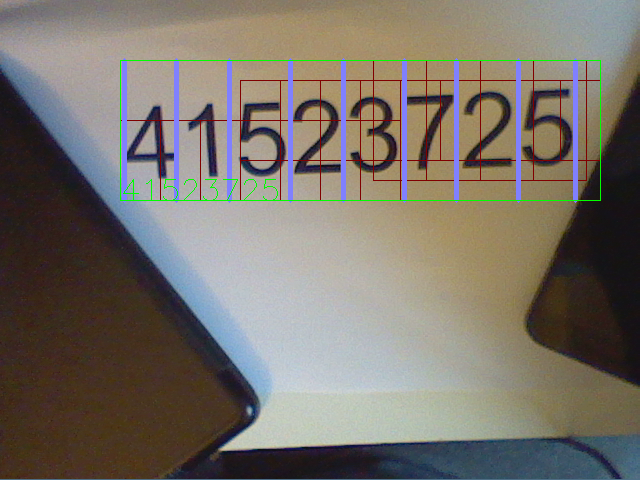
\includegraphics[width=0.5\linewidth]{fig/screenshots/0c64bcfc-61a5-4145-931e-1e68c99201c5}
      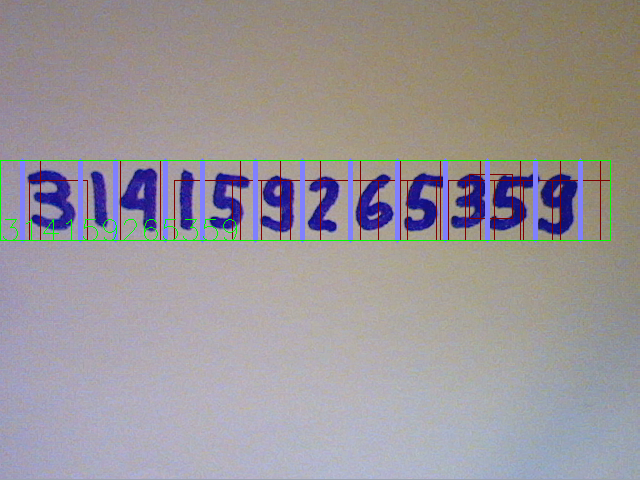
\includegraphics[width=0.5\linewidth]{fig/screenshots/33b6758a-5d0a-4725-8cef-74935f3d9174}
    }
    \caption
    {
      Screenshots of the proof-of-concept implementation of a text detection system using
      a webcam. Successful text detection (top left), reduced accuracy for rotated text (top right).
      Successful text detection in an image cluttered by high contrast edges (bottom left).
      Successful text detection of a handwritten number string (bottom right).
    }
    \label{fig:webcam}
\end{figure}

\section{Conclusion}
Implementing a photo OCR pipeline is a challenging problem. Not only do all of the different stages
of the pipeline have to achieve a high level of accuracy, their performance also has a direct
impact on the later stages. If, for example, the text detection stage does not extract a tightly
fitting bounding box, the segmentation and classification stages will receive character images
that are scaled down vertically, thus reducing their ability to perform at their maximum
accuracy.

Accuracy can be improved by increasing the spatial resolution and the number of intermediate scaling steps
of the sliding window text detection.
Both measures in turn will drastically increases the processing time per image. This problem is
further exacerbated if the system should also be able to extract text of small size because
this requires upscaling of the source image prior to text detection.

Apart from the unfavorable accuracy/time trade-off, the sliding window algorithm suffers from an additional
drawback: The text detection classifier has to make accurate decisions based only on the contents
of a small section of the whole image. All surrounding contextual information is discarded, which
makes it very hard to reach a high accuracy. Does an edge detected in a window belong to a character
or is it the edge of a piece of paper? Is there an arc of a digit or does the background have
some coarse structure to it? These dilemmas make it very hard
to implement a robust system that generalizes well over a broad range of applications and
would instead lead to specifically tuned versions for different purposes
(e.g. document scanning vs.\ extracting text from street view images).

Improving the sliding window algorithm could be achieved by dividing text detection into
multiple phases. In \cite{Li2016}, candidate bounding boxes are first computed using a
simple CNN classifier which are then further filtered on multiple resolutions
based on heuristics from the problem domain (car license plate detection). In \cite{Jaderberg2016},
proposals are filter using a random forrest classifier and then further enhanced using a regression
technique.

Overall it seems that the sliding window algorithm, while relatively straightforward to implement
(if hard to optimize) and widely used, would better be replaced by a solution that can be trained
end-to-end and that takes more image context into account. One technique are R-CNNs \cite{Girshick2013,Jaderberg2016},
which use a selective search in image space to generate proposal regions that are then fed
into a CNN for classification. Another technique is YOLO (You Only Look Once, \cite{Redmon}) that
uses a grid of classifiers in order to directly predict the position and size of bounding boxes.
Finally, if the (maximum) length of the text is known for the application \cite{Goodfellow2013,Li2016}, this will also greatly simplify
the detection algorithm as, for example, the aspect ratio of the text bounding boxes can be used
to filter out false positives.

\newpage
\bibliography{main,web}
\bibliographystyle{ieeetr}

\end{document}
